% !TeX encoding = windows-1251
\documentclass[12pt,a4paper]{article}
\usepackage[mag=980, tikz]{newlistok}

\УвеличитьШирину{1.5cm}
\УвеличитьВысоту{2.5cm}
% \renewcommand{\spacer}{\vspace{2pt}}

\ВключитьКолонтитул


\begin{document}


\Заголовок{Перечислительная комбинаторика -- 2}
\НадНомеромЛистка{179 школа, 7Б.}
\НомерЛистка{6}
\ДатаЛистка{27.09 -- 14.10 /2017}
\СоздатьЗаголовок


\пзадача
\пункт Разбейте все анаграммы слова {\tt ДЯдя} на группы, в которых все слова одинаковые, если не различать размер букв;
\пункт Разбейте все последовательности из 3 синих и 3 красных бусин в группы, в которых одинаковые ожерелья, если соединить последовательность в кольцо;
\пункт Как посчитать все анаграммы слова {\tt ДЯДЯ}?
\пункт Как посчитать количество ожерелий из 3 синих и 3 красных бусин?
\кзадача


\задача В классе учатся 20 человек. Сколькими способами из них можно
выбрать двоих школьников: старосту и ответственного за проездные билеты?
А просто двоих школьников?
\кзадача

\задача
Сколько разных слов (не только осмысленных) можно получить,
переставляя буквы в словах
\вСтрочку
\пункт
{\tt РОК};
\пункт
{\tt КУРОК};
\пункт
{\tt КОЛОБОК};
\пункт
$\underbrace{{\tt A}{\tt A}\dots{\tt A}}_a
\underbrace{{\tt B}{\tt B}\dots{\tt B}}_b$?
\спункт
$\underbrace{{\tt c}_1\dots{\tt c}_1}_{k_1}
\underbrace{{\tt c}_2\dots{\tt c}_2}_{k_2}
\,\dots\,\dots\,
\underbrace{{\tt c}_m\dots{\tt c}_m}_{k_m}$.
\кзадача

\задача
\пункт Сколькими способами можно выбрать трёх дежурных в классе
из 20 человек?\\
\пункт А сколькими способами можно выбрать старосту, его помощника
и трёх дежурных?
\кзадача

\опр \выд{Числом сочетаний из $n$ элементов по $k$} называется количество
способов выбрать $k$ предметов из $n$ различных предметов.
Обозначение: $n\choose k$
или $C_n^k$ (читается \лк це из $n$ по $k$\пк).
\копр

\пввзадача
Докажите, что
\вСтрочку
\пункт
$C_n^k=C_n^{n-k}$;
\пункт
$C_{n+1}^k=C_n^k+C_n^{k-1}$.
\кзадача

\пввзадача
Найдите формулу для $C_n^k$.
\кзадача

\УстановитьГраницы{0cm}{5.3cm}
\righttikz{0mm}{10mm}{
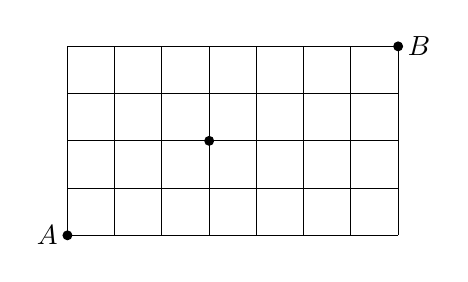
\begin{tikzpicture}[scale=0.6]
    \draw (0,0) grid (7, 4);
    \foreach \pt in {(0,0), (3,2), (7,4)} \fill \pt circle (3pt);
    \draw (0,0) node[left] {$A$} (7, 4) node[right] {$B$};
\end{tikzpicture}
}
\задача
\пункт
На рисунке справа изображен план города
(линии --- это~ули\-цы,  пересечения линий --- перекрестки).
На улицах~\hbox{введено} одностороннее движение: мож\-но
ехать только \лк вверх\пк\ или \лк впра\-во\пк. Сколько разных
маршрутов ведёт из точ\-ки $A$ в точ\-ку $B$?
\ВосстановитьГраницы
\пункт
Сколько из этих маршрутов не проходят через отмеченную на плане
точку внутри города?
\кзадача


\пзадача Сколькими способами можно рассадить класс,
если пришло 27 человек, а мест 30?
\кзадача

\задача
Сколькими способами можно высадить в ряд 3 груши и 4 яблони?
\кзадача

\УстановитьГраницы{0cm}{7.3cm}
\righttikz{-3mm}{5mm}{
$
\begin{array}{ccccccccccccc}
&&&&&&1\\
&&&&&1&&1\\
&&&&1&&2&&1\\
&&&1&&3&&3&&1\\
&&1&&4&&6&&4&&1\\
&1&&5&&10&&10&&5&&1\\
.&&.&&.&&.&&.&&.&&.
\end{array}
$}
\опр \выд{Треугольником Паскаля} называют числовой треугольник,
изображенный на рисунке справа (по краям треугольника стоят единицы,
а каждое из остальных чисел равно сумме двух, стоящих справа
и слева над ним).
\копр
\ВосстановитьГраницы


\УстановитьГраницы{0cm}{8cm}
\пзадача
На рисунке выписаны первые 6 строк треугольника Паскаля.
Напишите следующие 5 строк.
\кзадача
\ВосстановитьГраницы

\пзадача
Докажите, что $k$-ое число $n$-ой строки равно $C_n^k$
(строки нумеруются сверху вниз, начиная с нуля,
а числа в строках нумеруются слева направо, также начиная с нуля).
\кзадача

\пзадача
Докажите, что сумма чисел в $n$-ой строке треугольника Паскаля
равна~$2^n$.
\кзадача

\задача
Докажите тождество:
$C_n^1+2C_n^2+3C_n^3+\ldots+nC_n^n=n2^{n-1}$.
\кзадача

\ввзадача
\пункт Раскройте скобки и приведите подобные в выражениях
$(a+b)^2$, $(a+b)^3$, $(a+b)^4$.\\
\пункт [Бином Ньютона] Раскроем скобки и приведём подобные
в выражении $(a+b)^n$. Докажите, что любое слагаемое имеет вид $C\cdot a^k\cdot b^{n-k}$, причём $C=C_n^k$.\\
\пункт
Найдите коэффициенты при $x^{17}$ и $x^{18}$ после раскрытия
скобок и приведения подобных в $(1+x^5+x^7)^{20}$.
\кзадача

\задача
Докажите тождество: $C_n^0-C_n^1+C_n^2-C_n^3+\ldots+(-1)^nC_n^n=0$.
\кзадача

\задача
Возьмём любое число $C$ в треугольнике Паскаля и сложим все
числа, начиная с него и идя по прямой направо-вверх.
Докажите, что сумма равна числу, стоящему под $C$ справа.
%Запишите доказанное утверждение в виде тождества.
\кзадача

\задача
Из задачи 16 найдите суммы
\пункт
$T_n=1+\ldots+n$;
\пункт $П_n=T_1+\ldots+T_n$;
\пункт $П_1+\ldots+П_n$.
\кзадача

\сзадача
Как из предыдущей задачи вывести формулы для сумм  $1^2+\ldots+k^2$,
$1^3+\ldots+k^3$, \ldots?
\кзадача

\сзадача
Отметьте в треугольнике Паскаля чётные числа.
В каких строках %треугольника Паскаля
все числа нечётные?
\кзадача

\сзадача
Докажите, что
$C_p^0\cdot C_q^m+C_p^1\cdot C_q^{m-1}+\ldots+C_p^{m-1}\cdot C_q^1
+C_p^m\cdot C_q^0=C_{p+q}^m$.
\кзадача


% \vspace*{-2mm}
\ЛичныйКондуит{0mm}{6mm}
% \vspace*{-3mm}
%\GenXMLW

\end{document}

\vspace*{-0.2truecm}

\раздел{$***$}

\vspace*{-0.2truecm}

\задача
%\пункт
В НИИ работают 67 человек. Из них
47 знают английский язык, 35 --- немецкий, и 23 --- оба языка.
Сколько человек в НИИ
не знают ни английского, ни немецкого языков?
\пункт Пусть кроме этого  польский
знают 20 человек, английский и польский --- 12, немецкий и
польский --- 11, все три языка --- 5.
Сколько человек не знают ни одного из этих языков?
%\спункт [Формула включений и исключений]
%Решите задачу в общем случае: имеется $m$ языков,
%и для каждого набора языков известно, сколько человек знают все языки
%из этого набора.
\кзадача

\задача
В ряд записали 105 единиц, поставив перед каждой знак \лк$+$\пк.
Сначала изменили знак на противоположный перед каждой третьей единицей,
затем --- перед каждой пятой, а затем --- перед
каждой седьмой. Найдите значение полученного выражения.
\кзадача

\задача \вСтрочку
\пункт
На полке стоят 10 книг. Сколькими способами их можно переставить
так,~чтобы ни одна книга не осталась на месте?
\пункт А если на месте должны остаться ровно 3 книги?
\кзадача
